\section{Intro}
To understand the topic of signal processing, one must be familiar with the following topics:
\subsection{Euler's formula}
$$
e^{i x}=\cos x+i \sin x
$$
The derivation of Euler's formula can be found in the following \href{https://youtu.be/sKtloBAuP74}{video}.
% <iframe src="https://www.youtube.com/embed/sKtloBAuP74" title="YouTube video player" allow="accelerometer; autoplay; clipboard-write; encrypted-media; gyroscope; picture-in-picture" allowfullscreen="" width="560" height="315" frameborder="0"></iframe>
and the following:
% <iframe src="https://www.youtube.com/embed/v0YEaeIClKY" title="YouTube video player" allow="accelerometer; autoplay; clipboard-write; encrypted-media; gyroscope; picture-in-picture" allowfullscreen="" width="560" height="315" frameborder="0"></iframe>
This formula allows us to describe a signal in a very easy way.
\subsection{Convolution}
$$
\{f * g\}(t)=\int_{-\infty}^{+\infty} f(u) g(t-u) d u
$$
Note that the convolution has an identity element which is the $\delta(t)$ function, which's integral is one.
\subsection{Parseval's theorem}
Says that the energy in the time domain is the same as the energy in the frequency domain. Furthermore, it allows to see how the energy is distributed over different frequencies.
$$
E=\int_{-\infty}^{+\infty}|f(t)|^2 d t=\frac{1}{2 \pi} \int_{-\infty}^{+\infty}|F(\omega)|^2 d \omega=\int_{-\infty}^{\infty} E(\omega) d \omega
$$
\subsubsection{Energy Spectrum}
$$
E(\omega)=\frac{1}{2 \pi}|F(\omega)|^2
$$
\subsubsection{Energy in a frequency band}
$$
E\left(\omega_1 \leq \omega \leq \omega_2\right)=\int_{\omega_1}^{\omega_2} E(\omega) d \omega=\frac{1}{2 \pi} \int_{\omega_1}^{\omega_2}|F(\omega)|^2 d \omega
$$
\subsection{LTI Systems}
LTI means linear and time invariant. Which says that a linear combination of inputs generates the same linear combination of outputs and when I input a signal a little bit later into my system, I get the same output as if I would have entered the signal earlier. $\Rightarrow$ no new frequencies can be produced and when the input is band limited also the output must be band limited.
$$
a x_1(t)+b x_2(t) \Rightarrow a y_1(t)+b y_2(t)
$$
$$
x_1(t-\tau) \Rightarrow y_1(t-\tau)
$$
% <iframe src="https://www.youtube.com/embed/9fq5pUCHC8U" title="YouTube video player" allow="accelerometer; autoplay; clipboard-write; encrypted-media; gyroscope; picture-in-picture" allowfullscreen="" width="560" height="315" frameborder="0"></iframe>
\subsection{Fourier transform}
$$
\begin{aligned}
&F(\omega)=\int_{-\infty}^{\infty} f(t) e^{-i \omega t} d t \\
&f(t)=\frac{1}{2 \pi} \int_{-\infty}^{\infty} F(\omega) e^{i \omega t} d \omega
\end{aligned}
$$
% <iframe src="https://www.youtube.com/embed/spUNpyF58BY" title="YouTube video player" allow="accelerometer; autoplay; clipboard-write; encrypted-media; gyroscope; picture-in-picture" allowfullscreen="" width="560" height="315" frameborder="0"></iframe>
\subsection{Causality}
A causal system is one that at a specific time, the output is only a function of the input at that time or before (but never after)
Example of Casula systems:
$$
y(t)=R x(t)
$$
$$
y\left(t_0\right)=\frac{1}{C} \int_{-\infty}^{t_0} x(z) d z
$$
Example of a not casual system
$$
y\left(t_0\right)=\frac{1}{T} \int_{t_0-T / 2}^{t_0+T / 2} x(z) d z
$$

\subsection{Energy spectral density ESD}
\subsubsection{Autocorrelation function}
$$
R_x(\tau)=\int_{-\infty}^{\infty} x(t) x(t+\tau) d t \quad \text { for }-\infty<\tau<\infty
$$
The value at the origin of the autocorrelation is equal to the energy of the signal.
The energy spectral density is given by the following formula (see also parsevals theorem there is also the factor$2\pi$):
$$
E(\omega)=\frac{|F(\omega)|}{2 \pi}
$$
Note that the energy spectral density can also be calculated with the autocorrelation, as can be seen below:
$$
F^*(\omega) \cdot F(\omega)=|F(\omega)|^2=E(\omega)
$$

\subsection{Energy vs Power}
\begin{itemize}
\item All realistic signal are energy signals
\item All periodic signals are power signals
\item All random signals are power signals
\end{itemize}
$$
P=\lim _{T \rightarrow \infty} \frac{1}{T} \int_{-T / 2}^{+T / 2}|f(t)|^2 d t
$$
$$
E=\lim _{T \rightarrow \infty} \int_{-T / 2}^{+T / 2}|f(t)|^2 d t
$$

\subsection{Power spectral density PSD}
When we talk about a periodic signal, we talk about the power spectral density. It has a discrete power spectrum density.
$$
G_x(f)=\sum_{n=-\infty}^{\infty}\left|c_n\right|^2 \delta\left(f-n f_0\right)
$$
\section{Analytic Signal}
\subsection{Intro}
In a real valued signal there is redundant information in the negative-frequency part of the signal spectrum. Due to that, one can mask out the negative frequencies with the following formula:
$$
X_{\mathrm{a}}(f) \triangleq 2 \cdot \varepsilon(f) \cdot X(f)= \begin{cases}2 X(f) & f> 0 \\ X(f) & f=0 \\ 0 & f< 0\end{cases}
$$
As a result, one gets then the so-called analytic signal which lacks the symmetry properties in the Fourier transform and is therefore complex. $\varepsilon(f)$ is the Heaviside step function. To get the analytic signal one can use the Hilbert transform, which is the convolution of $x(t)$ with $h(t)=\frac{1}{\pi t}$. See the formula below:
$$
\begin{aligned}
x_{\mathrm{a}}(t) &=x(t) *\left(\delta(t)+j \cdot \frac{1}{\pi t}\right) \\
&=x(t)+j \cdot\left(x(t) * \frac{1}{\pi t}\right) \\
&=x(t)+j \cdot \mathcal{H}(x(t)) \\
&=x(t)+j \cdot \hat{x}(t),
\end{aligned}
$$
The Hilbert transforms frequency response can be found below, which is also called the hilbert filter.
$$
H(f)=-j \cdot \operatorname{sign}(f)= \begin{cases}-j & f>0 \\ 0 & f=0 \\ j & f<0\end{cases}
$$
The resulting analytic signal in the frequency domain is then the following:
$$
\begin{aligned}
X_{\mathrm{a}}(f)=\mathcal{F}\left(x_{\mathrm{a}}(t)\right) &=\mathcal{F}(x(t)+j \cdot \hat{x}(t)) \\
&=X(f)+j \cdot \hat{X}(f) \\
&=X(f)+j \cdot H(f) \cdot X(f) \\
&=X(f)+j \cdot(-j \operatorname{sign}(f)) \cdot X(f) \\
&=X(f) \cdot(1+\operatorname{sign}(f))= \begin{cases}2 X(f) & f>;0 \\
X(f) & f=0 \\
0 & f<0\end{cases}
\end{aligned}
$$
\begin{figure}[h]
    \begin{tikzpicture}
        \draw[->] (1,0) node [below]{$(-f_1)$} -- (1,1) node [above left] {$(\frac{A_0}{2})$};
        \draw[->] (7,0) node [below]{$(f_1)$} -- (7,1) node [above right] {$(\frac{A_0}{2})$};
        \draw[->] (4,0) node [below]{$0$} -- (4,2) node [above right] {$$};
        \draw[->] (0,0) -> (8,0) node [below right] {$f(\omega )$};
    \end{tikzpicture}
    \centering
    \caption{Cosine Spectrum}
\end{figure}
\begin{figure}[h]
    \begin{tikzpicture}
        \draw[->] (1,0) node [above]{$(-f_1)$} -- (1,-1) node [below left] {$(\frac{A_0}{2})$};
        \draw[->] (7,0) node [below]{$(f_1)$} -- (7,1) node [above right] {$(\frac{A_0}{2})$};
        \draw[->] (4,0) node [below]{$0$} -- (4,2) node [above right] {$$};
        \draw[->] (0,0) -> (8,0) node [below right] {$f(\omega )$};
    \end{tikzpicture}
    \centering
    \caption{Sine Spectrum}
\end{figure}
\subsubsection{Exercise Hilbert transform}
Let x(t) be a band limited signal whose spectrum $X(f)$ is limited to $-f_0 \leq f \leq f_0$
\begin{itemize}
    \item Compute the Hilbert transform of the band-pass signal
    $$
    \begin{aligned}
    \tilde{x}(t) & =A(t) \cos \left(2 \pi f_0 t+\phi(t)\right) \\
    & =A(t)\left[\cos \left(2 \pi f_0 t\right) \cos (\phi(t))-\sin \left(2 \pi f_0 t\right) \sin (\phi(t))\right] \\
    & =A(t) \cos (\phi(t)) \cos \left(2 \pi f_0 t\right)-A(t) \sin (\phi(t)) \sin \left(2 \pi f_0 f\right)
    \end{aligned}
    $$
    For a bandpass signal \autoref{eq:hilbert_bandpass} applys.
    \begin{equation}\label{eq:hilbert_bandpass}
    \begin{aligned}
    & \mathcal{H}\left(x(t) \cos \left(2 \pi f_0 t\right)\right)=x(t) \sin \left(2 \pi f_0 t\right) \quad \text { and } \\
    & \mathcal{H}\left(x(t) \sin \left(2 \pi f_0 t\right)\right)=-x(t) \cos \left(2 \pi f_0 t\right)
    \end{aligned}
    \end{equation}
    Therefore, the Hilbert transform is 
    $$
    \begin{aligned}
    \mathcal{H}(\tilde{x}(t)) & =A(t) \cos (\phi(t)) \sin \left(2 \pi f_0 t\right)+A(t) \sin (\phi(t)) \cos \left(2 \pi f_0 t\right) \\
    & =A(t) \sin \left(2 \pi f_0 t+\phi(t)\right)
    \end{aligned}
    $$
    Due to Ptolemy's identities, the sum and difference formulas for sine and cosine, which can be found in \autoref{eq:Ptolemy}.
    \begin{equation}\label{eq:Ptolemy}
    \begin{aligned}
    & \sin (\alpha+\beta)=\sin \alpha \cos \beta+\cos \alpha \sin \beta \\
    & \cos (\alpha+\beta)=\cos \alpha \cos \beta-\sin \alpha \sin \beta \\
    & \sin (\alpha-\beta)=\sin \alpha \cos \beta-\cos \alpha \sin \beta \\
    & \cos (\alpha-\beta)=\cos \alpha \cos \beta+\sin \alpha \sin \beta
    \end{aligned}
\end{equation}
    \item Compute the amplitude envelope of the signal $\tilde{x}(t)$\newline
    The analytic signal $x_a(t)$ of $\hat{x}(t)$ is
    $$
    \begin{aligned}
    x_a(t) & =\tilde{x}(t)+j \mathcal{H}(\tilde{x}(t)) \\
    & =A(t) \cos \left(2 \pi f_0 t+\phi(t)\right)+j A(t) \sin \left(2 \pi f_0 t+\phi(t)\right) .
    \end{aligned}
    $$
    And the amplitude envelope is
    $$
    \begin{aligned}
    \left|x_a(t)\right| & =|A(t)| \sqrt{\cos ^2\left(2 \pi f_0 t+\phi(t)\right)+\sin ^2\left(2 \pi f_0 t+\phi(t)\right)} \\
    & =|A(t)| .
    \end{aligned}
    $$
\end{itemize}
\section{CIC filter (Cascade-Integrator Comb)}
\href{https://www.dsprelated.com/showarticle/1337.php}{Cascaded integrator-comb (CIC)} digital filters are computationally-efficient implementations of narrowband lowpass filters, and are often embedded in hardware implementations of decimation, interpolation, and delta-sigma converter filtering. 

An example can be found in \autoref{fig:comp_filter_4}, where one sees it's low pass filter behaviour. As the name describes, a CIC filter is a cascade of an integrator ($\frac{1}{1-z^{-1}}$) and a comp($1-z^{-M}$) filter. The integrator is needed to cancel out the fist zero pole. The main advantage of this filter is described below (low computational effort) as well as the main disadvantage (nonlinearity).
\subsection{CIC Filter Applications}
CIC filters are well-suited for anti-aliasing filtering prior to decimation (sample rate reduction), as shown in \autoref{fig:cic_fig1}(a); and for anti-imaging filtering for interpolated signals (sample rate increase) as in \autoref{fig:cic_fig1}(b). Both applications are associated with very high-data rate filtering such as hardware quadrature modulation and demodulation in modern wireless systems, and delta-sigma A/D and D/A converters. 

\begin{figure}[!ht]
    \centering
    \includegraphics[width=0.8\textwidth]{images/CIC_Filter/CIC_digital_filters_fig1.png}
    \caption{CIC filter applications: (a) for decimation; (b) for interpolation.}
    \label{fig:cic_fig1}
\end{figure}
Because their frequency magnitude responses are sin(x)/x-like, CIC filters are typically followed, or preceded, by linear-phase lowpass tapped-delay line finite impulse response (FIR) filters whose tasks are to compensate for the CIC filter's non-flat passband. 

The \autoref{fig:cic_fig1} cascaded-filter architectures have valuable benefits. For example:
\begin{itemize}
    \item The FIR filters operate at reduced clock rates minimizing power consumption in high-speed hardware applications 
    \item CIC filters are popular in hardware devices; they need no filter coefficient data storage and require no multiplications. The arithmetic needed to implement CIC filters is strictly additions and subtractions only.
    \item Narrowband lowpass filtering can be attained at a greatly reduced computational complexity compared to using a single lowpass FIR filter. And this property is why CIC filters are so attractive in decimating and interpolating DSP systems.
\end{itemize}
\subsection{Recursive Running Sum Filter}
CIC filters originate from the notion of a recursive running sum filter, which is itself an efficient form of a nonrecursive moving averager. Recall the standard D-point moving-average process in \autoref{fig:cic_fig2}(a). There we see that D-1 summations (plus one multiply by 1/D) are necessary to compute the averager's y(n) output sequence.
\begin{figure}[!ht]
    \centering
    \includegraphics[width=0.8\textwidth]{images/CIC_Filter/CIC_digital_filters_fig2.png}
    \caption{D-point moving-average and recursive running sum filters.}
    \label{fig:cic_fig2}
\end{figure}
The D-point moving-average filter's time-domain output is expressed as 
\begin{equation}\label{eq:cic_1}
y(n)=\frac{1}{D}[x(n)+x(n-1)+x(n-2)+x(n-3)+\ldots+x(n-D+1)]
\end{equation}
where n is our time-domain index. The z-domain expression for this moving averager's output is 
\begin{equation}\label{eq:cic_2}
Y(z)=\frac{1}{D}\left[X(z)+X(z) z^{-1}+X(z) z^{-2}+\ldots+X(z) z^{-D+1}\right]
\end{equation}
while its z-domain $H_{\mathrm{MA}}(z)$ transfer function is 
\begin{equation}\label{eq:cic_3}
H_{\mathrm{MA}}(z)=\frac{Y(z)}{X(z)}=\frac{1}{D}\left[1+z^{-1}+z^{-2}+\ldots+z^{-D+1}\right]=\frac{1}{D} \sum_{n=0}^{D-1} z^{-n}
\end{equation}

We provide these equations not to make things complicated, but because they're useful. \autoref{eq:cic_1} tells us how to build a moving averager, and \autoref{eq:cic_3} is in the form used by commercial signal processing software to model the frequency-domain behavior of the moving averager. 


The next step in our journey toward understanding CIC filters is to consider an equivalent form of the moving averager, the recursive running sum filter depicted in Figure 2(b). Ignoring the 1/D scaling, there we see that the current input sample x(n) is added to, and the oldest input sample x(n-D) is subtracted from, the previous output average y(n-1). It's called 'recursive' because it has feedback. Each filter output sample is retained and used to compute the next output value. The recursive running sum filter's difference equation is

\begin{equation}\label{eq:cic_4}
y(n)=\frac{1}{D}[x(n)-x(n-D)]+y(n-1)
\end{equation}
having a z-domain $H_{\mathrm{RRS}}(z)$ transfer function of 
\begin{equation}\label{eq:cic_5}
H_{\mathrm{RRS}}(z)=\frac{Y(z)}{X(z)}=\frac{1}{D} \cdot \frac{1-z^{-D}}{1-z^{-1}}
\end{equation}

We use the same H(z) variable for the transfer functions of the moving average filter and the recursive running sum filter because their transfer functions are equal to each other! It's true. \autoref{eq:cic_3} is the nonrecursive expression, and \autoref{eq:cic_5} is the recursive expression, for a D-point averager. The mathematical proof of this can be found in Appendix B of Reference [1], but shortly I'll demonstrate that equivalency with in example. 

Here is why we care about recursive running sum filters: the standard moving averager in \autoref{fig:cic_fig2}(a) must perform D-1 additions per output sample. The recursive running sum filter has the sweet advantage that only one addition and one subtraction are required per output sample, regardless of the delay length D! This computational efficiency makes the recursive running sum filter attractive in many applications seeking noise reduction through averaging. Next we'll see how a CIC filter is, itself, a recursive running sum filter. 

\subsection{CIC Filter Structures}
If we condense the delay line representation and ignore the 1/D scaling in \autoref{fig:cic_fig2}(b) we obtain the classic form of a 1st-order CIC filter, whose cascade structure is shown in \autoref{fig:cic_fig3}.

\begin{figure}[!ht]
    \centering
    \includegraphics[width=0.8\textwidth]{images/CIC_Filter/CIC_digital_filters_fig3.png}
    \caption{D-point recursive running sum filter in a cascaded integrator-comb implementation.}
    \label{fig:cic_fig3}
\end{figure}

The feedforward portion of the CIC filter is called the comb section, whose differential delay is D, while the feedback section is typically called an integrator. The comb stage subtracts a delayed input sample from the current input sample, and the integrator is simply an accumulator. The CIC filter's time-domain difference equation is 
\begin{equation}
y(n)=x(n)-x(n-D)+y(n-1)
\end{equation}
and its z-domain transfer function is 
\begin{equation}
H_{\text {cIc }}(z)=\frac{Y(z)}{X(z)}=\frac{1-z^{-D}}{1-z^{-1}}
\end{equation}
To see why the CIC filter is of interest, first we examine its time-domain behavior, for D = 5, shown in \autoref{fig:cic_fig4}. If a unit impulse sequence, a unity-valued sample followed by many zero-valued samples, was applied to the comb stage, that stage's output is as shown in \autoref{fig:cic_fig4}(a). Think, now, what would be the output of the integrator if its input was the comb stage's impulse response. The initial positive impulse from the comb filter starts the integrator's all-ones output. Then, D samples later the negative impulse from the comb stage arrives at the integrator to zero all further CIC filter output samples. 

\begin{figure}[!ht]
    \centering
    \includegraphics[width=0.8\textwidth]{images/CIC_Filter/CIC_digital_filters_fig4.png}
    \caption{Single-stage CIC filter time-domain responses when D = 5}
    \label{fig:cic_fig4}
\end{figure}

The key issue is that the combined unit impulse response of the CIC filter, being a rectangular sequence, is identical to the unit impulse responses of a moving average filter and the recursive running sum filter. (Moving averagers, recursive running sum filters, and CIC filters are close kin. They have the same z-domain pole/zero locations, their frequency magnitude responses have identical shapes, their phase responses are identical, and their transfer functions differ only by a constant scale factor.) If you understand the time-domain behavior of a moving averager, then you now understand the time-domain behavior of the CIC filter in \autoref{fig:cic_fig3}. 

The frequency magnitude and linear-phase response of a D = 5 CIC filter is shown in \autoref{fig:cic_fig5}(a) and \autoref{fig:cic_fig5}(b) where the frequency fs is the input signal sample rate measured in Hz.
\begin{figure}[!ht]
    \centering
    \includegraphics[width=0.8\textwidth]{images/CIC_Filter/CIC_digital_filters_fig5.png}
    \caption{Characteristics of a single-stage CIC filter when D = 5.}
    \label{fig:cic_fig5}
\end{figure}
The CIC filter's frequency response, derived in Reference [1], is: 
\begin{equation}\label{eq:cic8}
H_{\mathrm{CIC}}\left(e^{j 2 \pi f}\right)=e^{-j 2 \pi f(D-1) / 2} \cdot \frac{\sin (2 \pi f D / 2)}{\sin (2 \pi f / 2)}
\end{equation}
If we ignore the phase factor in \autoref{eq:cic8}, that ratio of sin() terms can be approximated by a sin(x)/x function. This means the CIC filter's frequency magnitude response is approximately equal to a sin(x)/x function centered at 0 Hz as we see in \autoref{fig:cic_fig5}(a). (This is why CIC filters are sometimes called sinc filters.)

Digital filter designers like to see z-plane pole/zero plots, so I provide the z-plane characteristics of a D = 5 CIC filter in \autoref{fig:cic_fig5}(C), where the comb filter produces D zeros, equally spaced around the unit-circle, and the integrator produces a single pole canceling the zero at $z=1$. Each of the comb's zeros, being a Dth root of 1, are located at $z(m)=e^{i 2 p m / D}$, where $m=0,1,2, \ldots, D-1$, corresponding to a magnitude null in \autoref{fig:cic_fig5}(a).

The normally risky situation of having a filter pole directly on the z-plane's unit circle need not trouble us here because there can be no coefficient quantization error in our $H_{\mathrm{CIC}(z)}$ transfer function. That's because CIC filter coefficients are ones and can be represented with perfect precision with fixed-point number formats. The filter pole will never be outside the unit circle. Although recursive, happily CIC filters are guaranteed-stable, linear-phase, and have finite-length impulse responses.

Again, CIC filters are primarily used for anti-aliasing filtering prior to decimation, and for anti-imaging filtering for interpolated signals. With those notions in mind we swap the order of \autoref{fig:cic_fig2}(C)'s comb and integrator-we're permitted to do so because those operations are linear-and include decimation by an integer sample rate change factor R in \autoref{fig:cic_fig6}(a). (The reader should prove to themselves that the unit impulse response of the integrator/comb combination, prior to the sample rate change, in \autoref{fig:cic_fig6}(a) is equal to that in \autoref{fig:cic_fig4}(C).) In most CIC filter applications the rate change R is equal to the comb's differential delay D, but I'll keep them as separate design parameters for now.

\begin{figure}[!ht]
    \centering
    \includegraphics[width=0.8\textwidth]{images/CIC_Filter/CIC_digital_filters_fig6.png}
    \caption{Single-stage CIC filters used in (a) decimation and (b) interpolation. (Sample rates $f_{s,in}$ and $f_{s,out}$ are the sample rates of the x(n) and y(n) sequences respectively.)}
    \label{fig:cic_fig6}
\end{figure}

The decimation (also called 'down-sampling') operation $\downarrow$R means discard all but every Rth sample, resulting in an output sample rate of $f_{s,out}$ = $f_{s,in}$/R. To investigate a CIC filter's frequency-domain behavior in more detail, \autoref{fig:cic_fig7}(a) shows the frequency magnitude response of a D=8 CIC filter prior to decimation. The spectral band, of width B Hz, centered at 0 Hz is the desired passband of the filter. A key aspect of CIC filters is the spectral folding that takes place due to decimation.

\begin{figure}[!ht]
    \centering
    \includegraphics[width=0.8\textwidth]{images/CIC_Filter/fig 7_83485.jpg}
    \caption{Magnitude response of a 1st-order, D=8, decimating CIC filter: (a) before decimation; (b) aliasing after R=8 decimation. )}
    \label{fig:cic_fig7}
\end{figure}

Those B-width shaded spectral bands centered about multiples of fs,in/R in \autoref{fig:cic_fig7}(a) will alias directly into our desired passband after decimation by R = 8 as shown in \autoref{fig:cic_fig7}(b). Notice how the largest aliased spectral component, in this 1st-order CIC filter example, is 16 dB below the peak of the band of interest. Of course the aliased power levels depend on the bandwidth B; the smaller B the lower the aliased energy after decimation.

\autoref{fig:cic_fig6}(b) shows a CIC filter used for interpolation where the $\uparrow$R symbol means insert R-1 zeros between each x(n) sample (up-sampling), yielding a y(n)output sample rate of $f_{s,out}=R\cdot f_{s,in}$. (In this CIC filter discussion, interpolation is defined as zeros-insertion, called 'zero stuffing', followed by CIC filter lowpass filtering.)

To illustrate the spectral effects of interpolation by R=8, \autoref{fig:cic_fig8}(a) shows an arbitrary baseband spectrum, with its spectral replications, of a signal applied to the D=R=8 interpolating CIC filter of \autoref{fig:cic_fig6}(c). The interpolation filter's output spectrum in \autoref{fig:cic_fig8}(b) shows how imperfect CIC filter lowpass filtering gives rise to the undesired spectral images. 
\begin{figure}[ht]
    \centering
    \includegraphics[width=0.8\textwidth]{images/CIC_Filter/fig 8_16431.jpg}
    \caption{1st-order, D=R=8, interpolating CIC filter spectra: (a) input signal spectrum; (b) spectral images of a zero stuffed and CIC lowpass filtered output.}
    \label{fig:cic_fig8}
\end{figure}

After interpolation, \autoref{fig:cic_fig8}(b) shows the unwanted images of the B-width baseband spectrum reside at the null centers, located at integer multiples of $f_{s,out}$/R. If we follow the CIC filter with a traditional lowpass tapped-delay line FIR filter, whose stopband includes the first image band, fairly high image rejection can be achieved.

\subsubsection{Comb Filters summary}
Moving average filter:
$$
H(z)=\sum_{k=0}^{M-1} z^{-k}
$$
This filter can also be written in IIR form which is the CIC filter:
$$
H(z)=\sum_{k=0}^{M-1} z^{-k}=\frac{1-z^{-M}}{1-z^{-1}}
$$
when using $z=\mathrm{e}^{j \omega T_s}$ we get the following result:
\begin{equation}\label{eq:CIC_filter_supression}
\begin{aligned}
H(f) &=\frac{1-\mathrm{e}^{-j \omega T_s \cdot M}}{1-\mathrm{e}^{-j \omega T_s}} \\
&=\frac{\mathrm{e}^{-j \frac{\pi f}{f_s} M}\left(\mathrm{e}^{j \frac{\pi f}{f_s} M}-\mathrm{e}^{-j \frac{\pi f}{f_s} M}\right)}{\mathrm{e}^{-j \frac{\pi f}{f_s}}\left(\mathrm{e}^{j \frac{\pi f}{f_s}}-\mathrm{e}^{-j \frac{\pi f}{f_s}}\right)} \\
&=\mathrm{e}^{-j \frac{\pi f}{f_s}(M-1)} \cdot \frac{\sin \left(\frac{\pi f}{f_s} M\right)}{\sin \left(\frac{\pi f}{f_s}\right)}
\end{aligned}
\end{equation}
When one cascades the filter, one gets the following formula: $Rightarrow$ The benefit is that one has more attenuation.
$$
H(z)=\left(\frac{1-z^{-M}}{1-z^{-1}}\right)^n
$$
With the command \mintinline[bgcolor=black]{matlab}{filterDesigner} one can open the filter Designer where one can set poles and zeros.\newline
\begin{listing}[!ht]
\begin{minted}[
frame=lines,
framesep=2mm,
baselinestretch=1.2,
bgcolor=black,
fontsize=\footnotesize,
linenos,
breaklines
]{matlab}
clc
clear
close all;
h_en = [1 -1];
impz(h_en,1,10);    %h_en = numerator, 1 = denumerator, 10 number of samples for impulse response
title({'\fontsize{14}{0}\selectfont Impulse Response','\fontsize{12}{0}\selectfont $X(z)=1-z^{-1}$'},'interpreter','latex');
[hz1, hp1, ht1] = zplane(h_en,1);%with the unit circle
set(findobj(hz1, 'Type', 'line'), 'Color', 'b','LineWidth',2); 
set(findobj(hp1, 'Type', 'line'), 'Color', [0, 0.7, 0],'LineWidth',2);
saveas(gcf,'C:\Users\...\impulse_response_1','epsc')

clc
[hz1, hp1, ht1] = zplane(h_en,1);%with the unit circle
set(findobj(hz1, 'Type', 'line'), 'Color', 'b','LineWidth',2); 
set(findobj(hp1, 'Type', 'line'), 'Color', [0, 0.7, 0],'LineWidth',2);
title({'\fontsize{14}{0}\selectfont Pole-Zero plot','\fontsize{12}{0}\selectfont $X(z)=1-z^{-1}=\frac{z-1}{z}$'},'interpreter','latex');
saveas(gcf,'C:\Users\...\pole_zero_1','epsc')

clc
freqz(h_en,1);
title({'Frequency response','$X(z)=1-z^{-1}$'},'interpreter','latex');
ax1 = gca; % current axes
ax1.Position(4) = ax1.Position(4)*.80; 
saveas(gcf,'C:\Users\...\freq_res_1','epsc')
\end{minted}
\end{listing}
\begin{figure}
\centering
\begin{subfigure}{.5\linewidth}
\centering
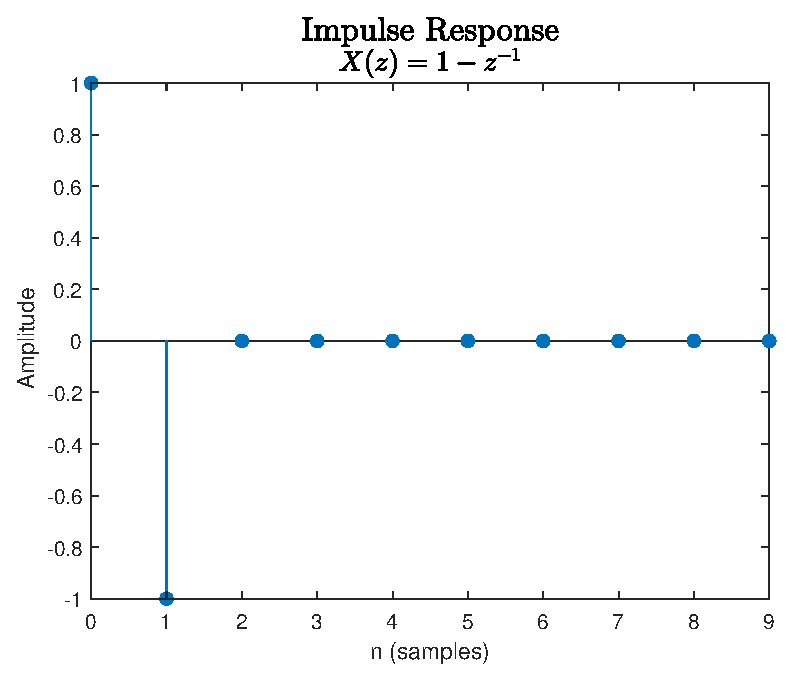
\includegraphics[scale=0.45]{images/impulse_response_1.eps}
\caption{}
\label{fig:sub1}
\end{subfigure}%
\begin{subfigure}{.5\linewidth}
\centering
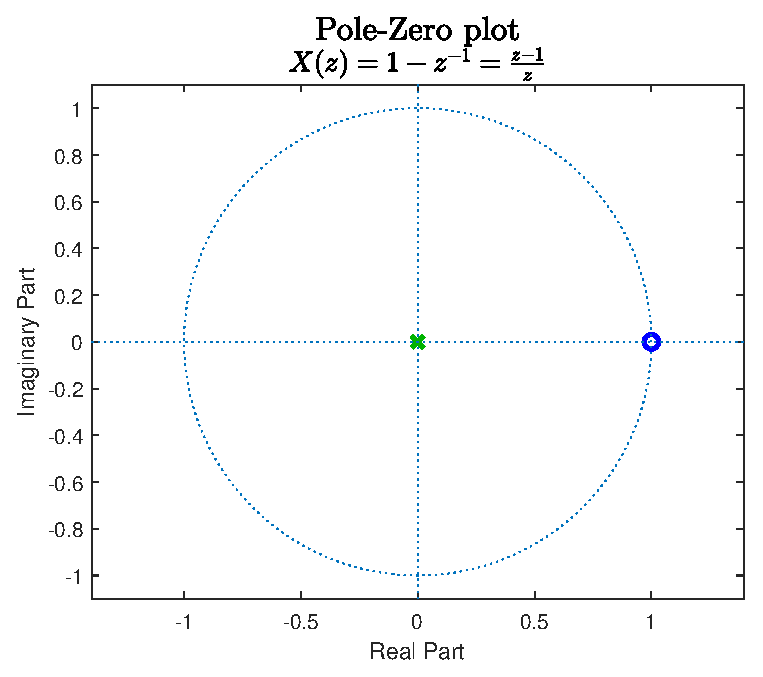
\includegraphics[scale=0.45]{images/pole_zero_1.eps}
\caption{}
\label{fig:sub2}
\end{subfigure}\\[1ex]
\begin{subfigure}{\linewidth}
\centering
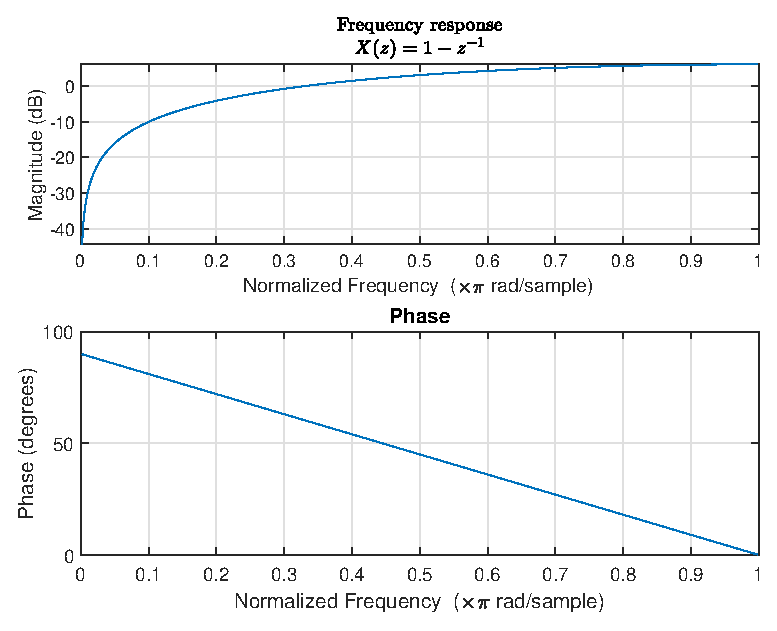
\includegraphics[scale=0.9]{images/freq_res_1.eps}
\caption{}
\label{fig:sub3}
\end{subfigure}
\caption{FIR filter}
\label{fig:test}
\end{figure}

\begin{figure}
\centering
\begin{subfigure}{.5\linewidth}
\centering
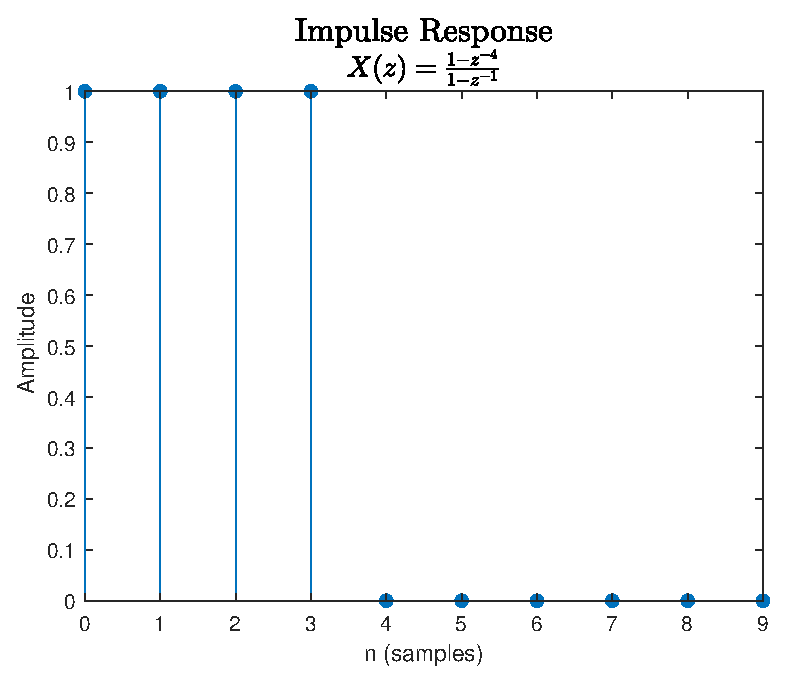
\includegraphics[scale=0.45]{images/impulse_response_2.eps}
\caption{}
\label{fig:sub1}
\end{subfigure}%
\begin{subfigure}{.5\linewidth}
\centering
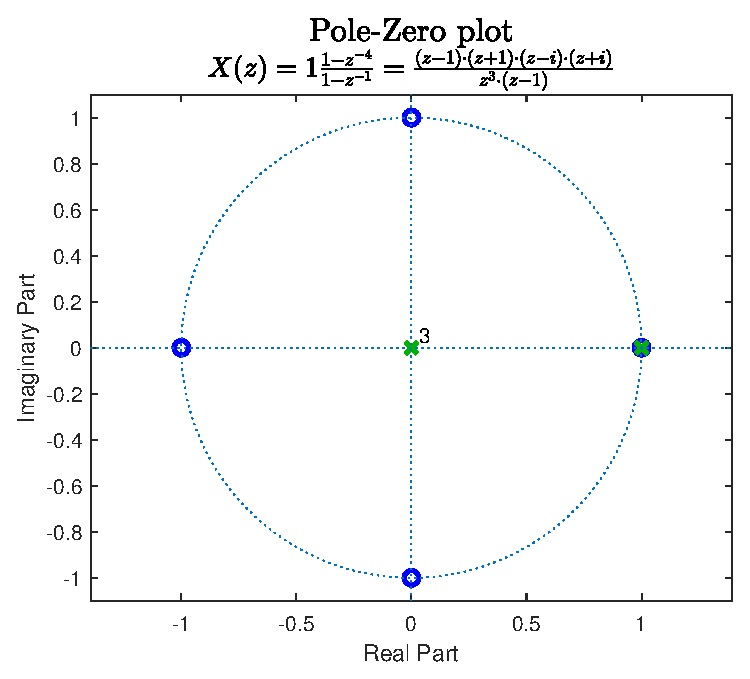
\includegraphics[scale=0.45]{images/pole_zero_2.eps}
\caption{}
\label{fig:sub2}
\end{subfigure}\\[1ex]
\begin{subfigure}{\linewidth}
\centering
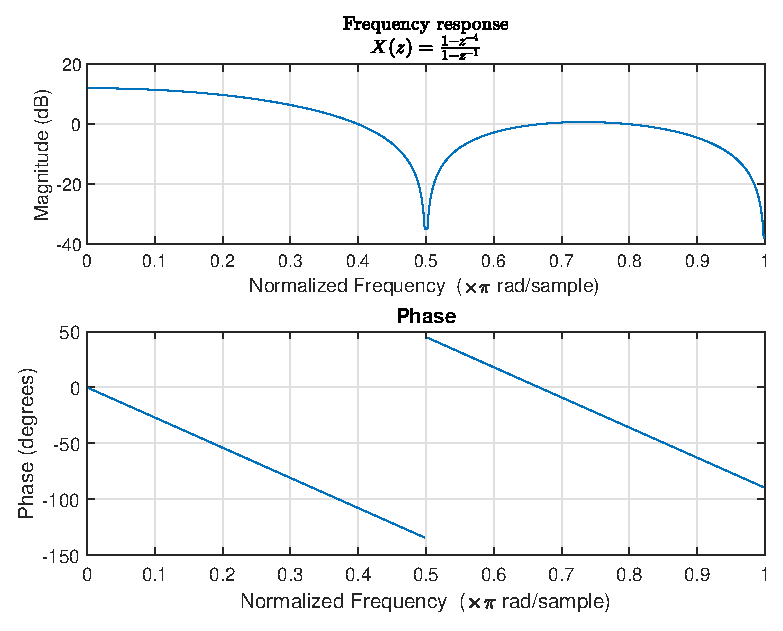
\includegraphics[scale=0.9]{images/freq_res_2.eps}
\caption{}
\label{fig:sub3}
\end{subfigure}
\caption{CIC filter with $M=4$, \textcolor{green}{Poles},\textcolor{blue}{Zeros}}
\label{fig:comp_filter_4}
\end{figure}


% \begin{figure}
%     \centering
%     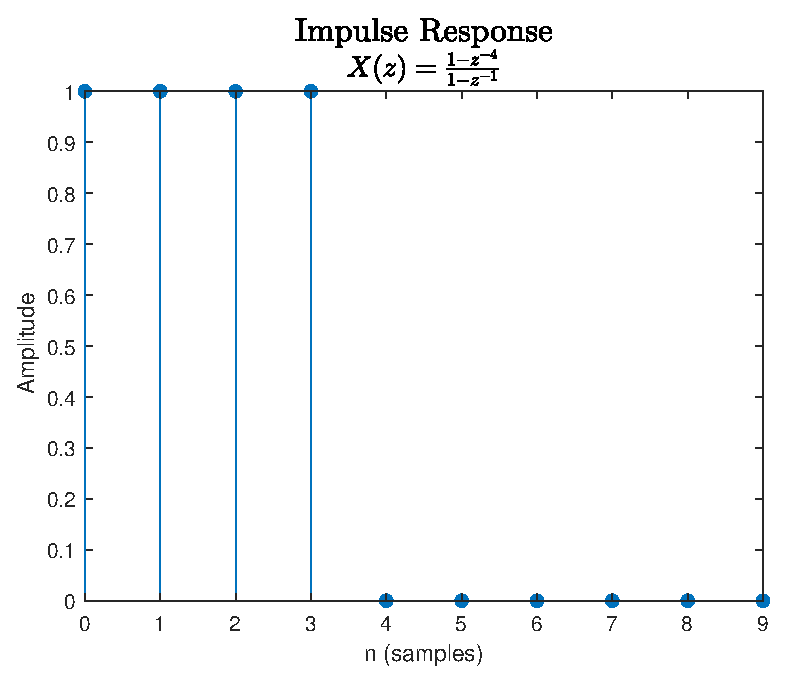
\includegraphics[scale=0.8]{images/impulse_response_2.eps}
%     \caption{Caption}
%     \label{fig:my_label}
% \end{figure}
% \begin{figure}
%     \centering
%     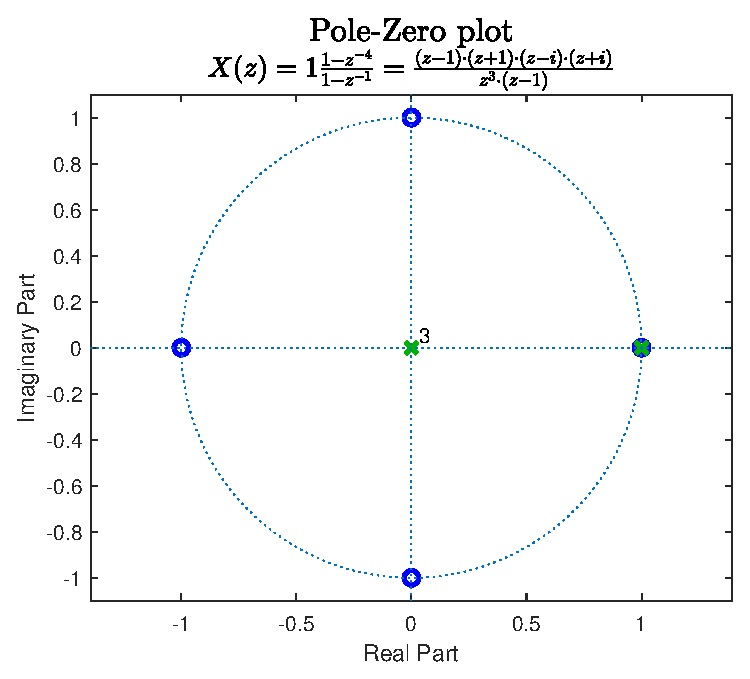
\includegraphics[scale=0.8]{images/pole_zero_2.eps}
%     \caption{Caption}
%     \label{fig:my_label}
% \end{figure}
% \begin{figure}
%     \centering
%     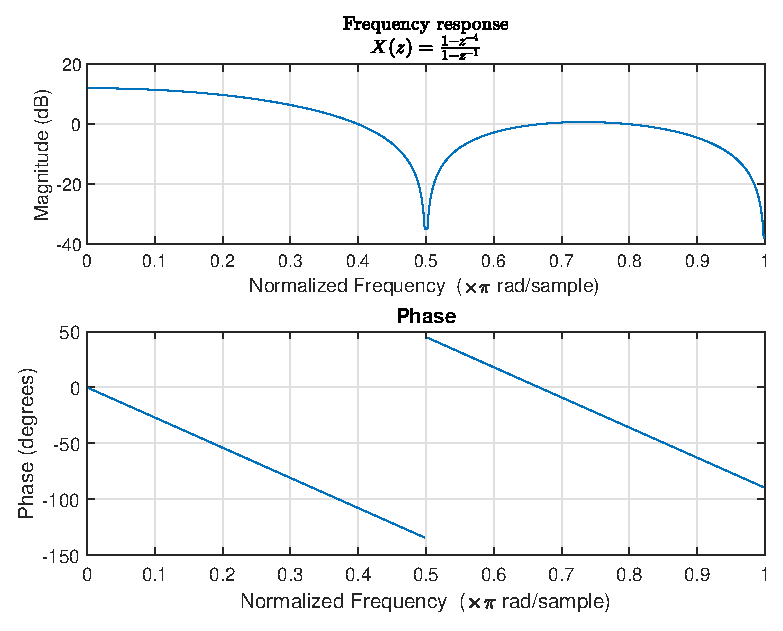
\includegraphics[scale=1]{images/freq_res_2.eps}
%     \caption{Caption}
%     \label{fig:my_label}
% \end{figure}
\FloatBarrier
\subsubsection{Exercise CIC filter}
In a digital receiver, the baseband signal is sampled with  $f_s = \SI{100}{\mega\hertz}$. To reduce the signal processing load
of the following stages, you design a CIC filter with M = 5 to bring the sampling rate down to $\SI{20}{\mega\hertz}$. The
corner frequency of the band of interest is at $f_c = \SI{5}{\mega\hertz}$.
\begin{itemize}
    \item At which frequency does the largest possible aliasing interfering with the band of interest occur? (Assuming white noise outside the band of interest.)\newline
    The largest alias occurs at the first aliasing frequency of the passband corner frequency $f_c$, i.e. $f_{a, \max }=\frac{f_s}{M}-f_c=15 \mathrm{MHz}$ (Since we downsample with a factor of five, our new sampling rate is 20MHz $\Rightarrow$ The frequency of 15MHz is read as the same as the frequency of 5MHz, 25MHz would also be an alias frequency, but is allready damped more)
    
    \item What is the minimum order n of the CIC filter to achieve an alias suppression greater than 40 dB?
    According to \autoref{eq:CIC_filter_supression} the following holds: $H(f)=e^{-j \frac{\pi f}{f_s} n(M-1)} \cdot\left(\frac{\sin \left(\frac{\pi f}{f_s} M\right)}{M \sin \left(\frac{\pi f}{f_s}\right)}\right)^n$. When one says that $H(f)$ at $f_a$ must be -40 db one gets the following for n: 
    $$\text{solve} \left(\left| e^{-j \frac{\pi \SI{15}{\mega\hertz}}{\SI{100}{\mega\hertz}} n(5-1)} \cdot\left(\frac{\sin \left(\frac{\pi \SI{15}{\mega\hertz}}{\SI{100}{\mega\hertz}} 5\right)}{5 \sin \left(\frac{\pi \SI{15}{\mega\hertz}}{\SI{100}{\mega\hertz}}\right)}\right)^n\right| = 10^{\frac{-40}{20}}\text{, n} \right)\Rightarrow n=3.94$$ Therefore the Order must be at least 4.
    \item How large is the passband droop for a filter of this order at $f_c$?\newline
    The drop at the passband is $\left| e^{-j \frac{\pi \SI{5}{\mega\hertz}}{\SI{100}{\mega\hertz}} n(5-1)} \cdot\left(\frac{\sin \left(\frac{\pi \SI{5}{\mega\hertz}}{\SI{100}{\mega\hertz}} 5\right)}{5 \sin \left(\frac{\pi \SI{5}{\mega\hertz}}{\SI{100}{\mega\hertz}}\right)}\right)^n\right|=0.668\Rightarrow 20\cdot \log_{10} 0.668=-3.5dB=H(f_c)$
\end{itemize}


